\begin{figure*}
\centering
%  \fbox{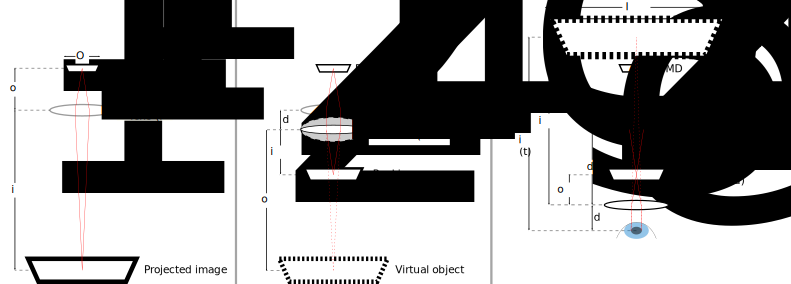
\includegraphics[width=0.46\textwidth]{images/volumetric/unfolded}}
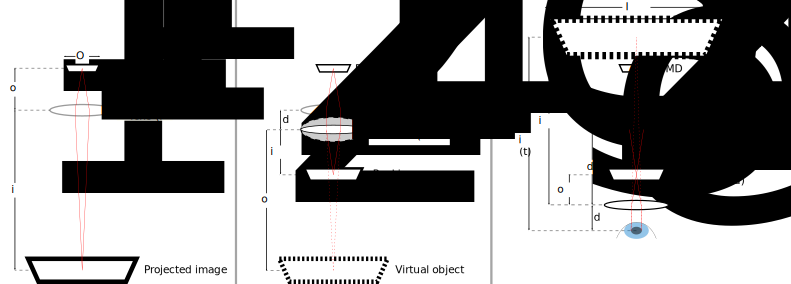
\includegraphics[width=0.95\textwidth]{images/volumetric/unfolded}
\caption[Volumetric NED: unfolded optics]{Our NED's optics can be analyzed in three stages. Figure shows the unfolded optics and ray diagram for each stage. \emph{Left: } Image formation for the DMD projector using manufacture-provided projection optics. \emph{Middle: } Adding a focus-tunable lens at the exit pupil of the DMD projector causes the real image of the DMD to be formed closer; Configuring the focus-tunable lens power to continuously oscillate causes the real image of the DMD to also oscillate. \emph{Right: } A combiner lens finally creates a virtual image of the DMD that can be seen by the eye.}
\label{fig:volumetric:unfolded}
\end{figure*}

